\section{The macro status in China and the potential opportunity and risk for the World}

\begin{enumerate}[1.]
    \item China has woke up and become an integral part of the world
    \item China is an old superpower with recent brief dent (How China
        fell and woke up)
    \item China is a Confucuius dominant contry (East and West culture
        difference)
    \item China is internally highly heterogenous and compley
\end{enumerate}

Why do we need to know about China?

\begin{itemize}
    \item As an entrepreneur, you may want to know the largest market in
        the world and see how to make money from Chinese.
    \item As a global citizen, you may want to know how the world is becoming
        more polarized as the rising of China, which is one of the major
        hotspots of challenges and innovations.
    \item As a potential partner or competitor, you may want to know your
        team member or your enemy better.
    \item "If you know the enemy and know yourself, you need not fear the
        results of hundred battles. If you know yourself but not the enemy,
        for every victory gained you will also suffer a defeat. If you know
        neither the enemy nor yourself, you will succumb in every battle."
\end{itemize}

Status after Covid-19.

\begin{table}[h]
    \centering
    \begin{tabular}{|c|c|}
        \hline
        US (and also Europe to dome degree) & China \\ \hline
        New budget and monetary experiment to stimulate &
        Curb government spending and are constraining \\
        final demand & money supply growth \\ \hline
        Launch massive investment programs at a time when &
        Rein in government spendint \\
        there is little industrial spare capacity & \\ \hline
        Encourage a property and constructoin boob, even as &
        Slow construction activity \\
        the sector suffers shortage of workers and raw materials & \\ \hline
    \end{tabular}
\end{table}

China's economic politymakers are using the space afforded them by a rapid
economic recovery from the pandemic to refocus on a longer-term effort to
redirect resources for strategic and political purmoses.

\vspace{1\baselineskip}

Excess money. The idea is that over long term money supply should grow at
roughly the same rate as nominal GDP. As a result, the ratio between the
growth of excess money in two economies should indicate which way the
exchange rate is heading - with the country showing the faster increase
in excess money supply having the weaker currency.

\paragraph{Cyclical strength means short-term growth is not a worry}

Even after accounting for base effects, cyclical growth drivers boomed in
1Q21. Exports and property sales grew even faster then pre-Covid rates.
Only consumption lagged, thanks to renewed public-health restrictions,
but should recover quickly. The first quarter was probably the cyclical peak,
and both reported and underlying growth will decelerate. Still, exports and
property sales have been stronger than expected, so momentum is solid.

\vspace{1\baselineskip}

Favorable base effects and the strong cyclical bounce mean the government's
deliberately low target of "above $6\%$" GDP growth in 2021 will be easily
met; consensus forecast are for $8.5\%$. Provincial governments' growth
targets are also quite conservative, as reduced urgency for growth has
percolated down. The government began withdrawing emergency counter-cyclical
support as early as mid-2020, and is continuing to do so in 2021.

\paragraph{Monetary and fiscal policy is tightening}

The turn in China's credit cycle is now well established, with total
credit growth slowing to $12.3\%$ YoY in March from the peak of $13.6\%$
in October. The apparent sharp slowdown in March was due to base effects,
not aggressive tightening; two-year growth shows a more moderate trejectory.
But regulators are hawkish, and their reported plan to cap new loans this
year implies total credit growth of $\sim 11\%$ for 2021, and possibly less.

\vspace{1\baselineskip}

The budgeted slowdown in total fiscal spending to just $4.9\%$ in 2021 is
a conservative signal to agencies and localities. Reduced fiscal support and
the slowing credit cycle shows much less political urgency on supporting
growth, and a higher priority on consolidating public finances. Since
public sector investment was already weak in 2020, further weakness will not
be a shock to growth. And incentives for new private investment are strong.

\paragraph{Environmental rules are tightening}

Another set of long-term priorities now getting a lot of short-term focus
are those around energy and the environment. Top leader Xi Jinping has
promised to cap China's carbon emissions by 2030 and achieve carbon
neutrality by 2060. Many projections suggest the 2030 goal as achievable
given recent rapid progress on renewable energy. But Xi's pledges have
nontheless led to a major shift in the policy envoronment.

\vspace{1\baselineskip}

Another trigger for tougher environmental enforcement was the 1Q21
resurgence in air pollution, particularly in north China (aggravated
by a dramatic dust storm). The Covid collapse curbed heavy-industry
emissions and the rebound is boosting them again. In previous air-quality
campaigns the government has used forced reductions in steel output to
produce pollution, and the steel sector is once again in policymakers'
crosshairs.

\paragraph{Statistics to China and Switzerland}
See Lecture Slides pages 10-14. \footnote{\url{https://xyotta.com/cfiles/1205}}


\subsection{China has woke up and become and integral part of the world}

\begin{figure}[h]
    \centering
    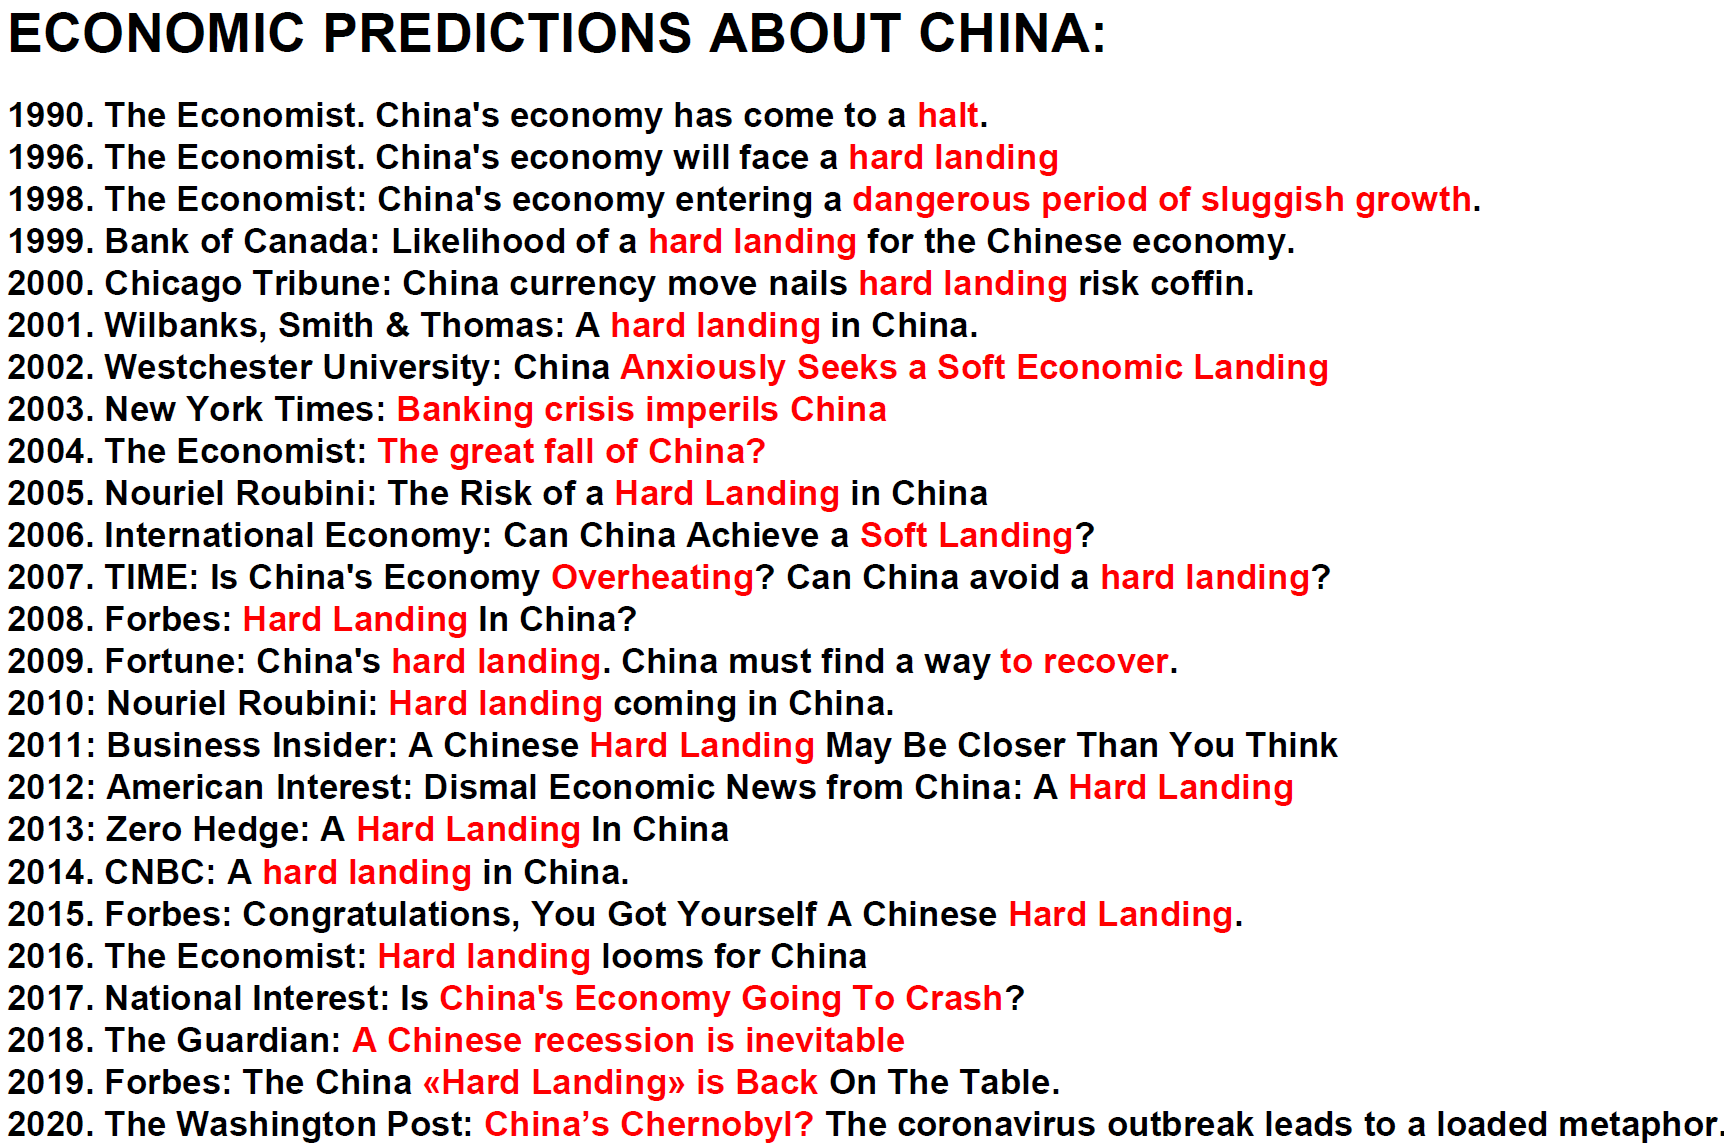
\includegraphics[width=0.8\textwidth]{Pictures/China_economic_prediction.png}
\end{figure}

\begin{itemize}
    \item GDP rose from $367.9$ billion yuan in 1978 to 99.1 trillion yuan
        (\$14.4 trillion) in 2019.
    \item Since 2010, China surpassed Japan and has become the second-largest
        economy in the world, accounting for around 16 percent of world economy
        in 2019 (30\% of world's economy growth), up 14 percentage points from
        1978.
    \item In 2013, China's GDP in purchasing power parity (PPP) terms overtook
        the USA's in 2013, and now accounts for nearly 19\% of global economy
    \item Per-capita GDP rose from 385 yuan (\$229) in 1978 to 70892 (\$10276)
        in 2019, lifting China from the notch of world's low-income to
        middle-income countries.
\end{itemize}

\paragraph{The government favors hardware over software}

Behind the hard line towards internet companies is a rethinking of which
sectors really matter for national progess. China's government is now convinced
that manufacturing matters more. Unlike the US, China does not see its internet
companies as leaders of national innovation, but as sources of social problems.
Internet entrepreneurs will get even more generous subsidies.

\vspace{1\baselineskip}

The current regulatory shift therefore is not negative for all Chinese listed
companies, or even all technology companies. Policy support for strategically
important sectors is ramping up, but most of those are hardware rather than
software: most prominently, semiconductors and renewable energy. Hardware
tech companies stock prices have done better than those of international
platforms in recent weeks, which could be the start of a trend.

\vspace{1\baselineskip}

In 1981, three years after Deng's reform project was launched, almost 90\%
of chinese people lived in extreme poverty by the definition of the World
Bank (\$1.9 per day). By 2016, that number had dropped to less than 0.5\%.
By the end of 2020, it is 0.

\vspace{1\baselineskip}

2016 the world's largest radio telescope with a folded aperture in China
was completed. The so-called FAST is a spherical radio telescope with a
diameter of 500 meters. It began its work in Guizhou Province.

\vspace{1\baselineskip}

In 2006, the Qinghai-Tibet Railway began oberations on the world's highest
railway line, at an average elevation around 4500m above sea level. Tanggula
railway station at 5068m is the world's highest railway station.

\vspace{1\baselineskip}

The third fastest supercomputer in the world as of Nov 2019. The Sunday
TaihuLight was the world's fastest supercomputer for two years, from June
2016 to June 2018, according to the TOP500 lists. The record was surpassed
in June 2018 by IBM's Summit.

\vspace{1\baselineskip}

\begin{itemize}
    \item With progress on urbanization and industrialization, more jobs
        were created in urban areas, from 2.6 million new jobs in 2000 to
        13.52 million in 2019.
    \item Total energy output rose from 627.7 million tons of standard coal
        in 1978 to 3.75 billion tons of standard coal in 2017.
    \item From 1978 to 2017, China's state revenue increased from 113.2 billion
        to 17 trillion yuan.
    \item China's retail sales of consumer goods grew from 155.9 billion yuan
        in 1978 to 41.16 trillion yuan in 2019.
    \item China's foreign trade volume rose from \$20.6 billion in 1978 to
        \$4.1 trillion in 2017. About 58.52\% of people lived in towns and
        cities in 2017, compared to 17.92\% back in 1978.
    \item China's high-speed railway developed from nothing. Up to 2017, the
        high-speed railway network covered 25000 km.
    \item Auto industry has witnessed an uptrend in production over the past
        40 years. The volume hit 29.02 million in 2017, up from 149000 back
        in 1978.
\end{itemize}

China has been one of the major driving forces in the world.

\vspace{1\baselineskip}

Chinese visitors account for a rising share of visitory and tourist spending
in many economies.

\vspace{1\baselineskip}

China is the world's anufacturing superpower.

\begin{itemize}
    \item China accounts for 30\% of global manufacturing output.
    \item Although it accounts for only 10\% of global houshold consumption,
        it was the source of 31\% of global houshold consumption growth from
        2010 to 2017.
    \item In many categories including automobiles, spirits, luxury goods,
        and mobile phones, China is the largest market in the world,
        accounting for about 30\% of global consumption.
    \item The world's second-largest source and second-largest recipient
        of FDI between 2015 and 2017.
\end{itemize}

China is so interconnected with other nations in trade that blocking china
as a trade partner would also cause effects for third countries.

\begin{figure}[H]
    \centering
    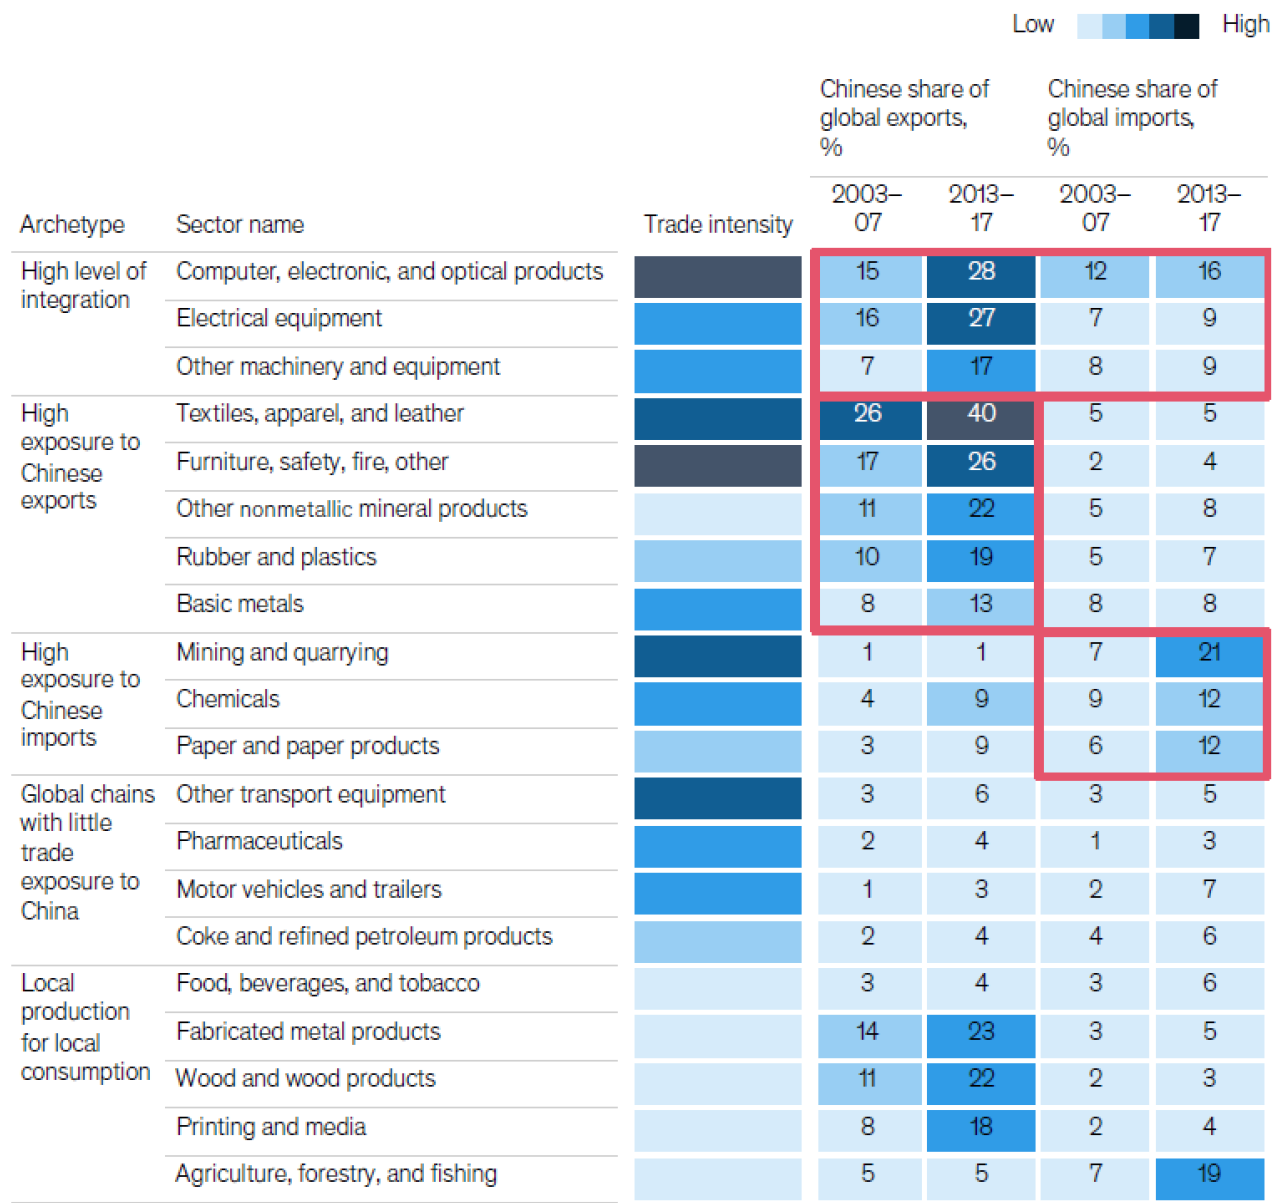
\includegraphics[width=0.75\textwidth]{Pictures/china_trade_1.png}
\end{figure}

\begin{figure}[H]
    \centering
    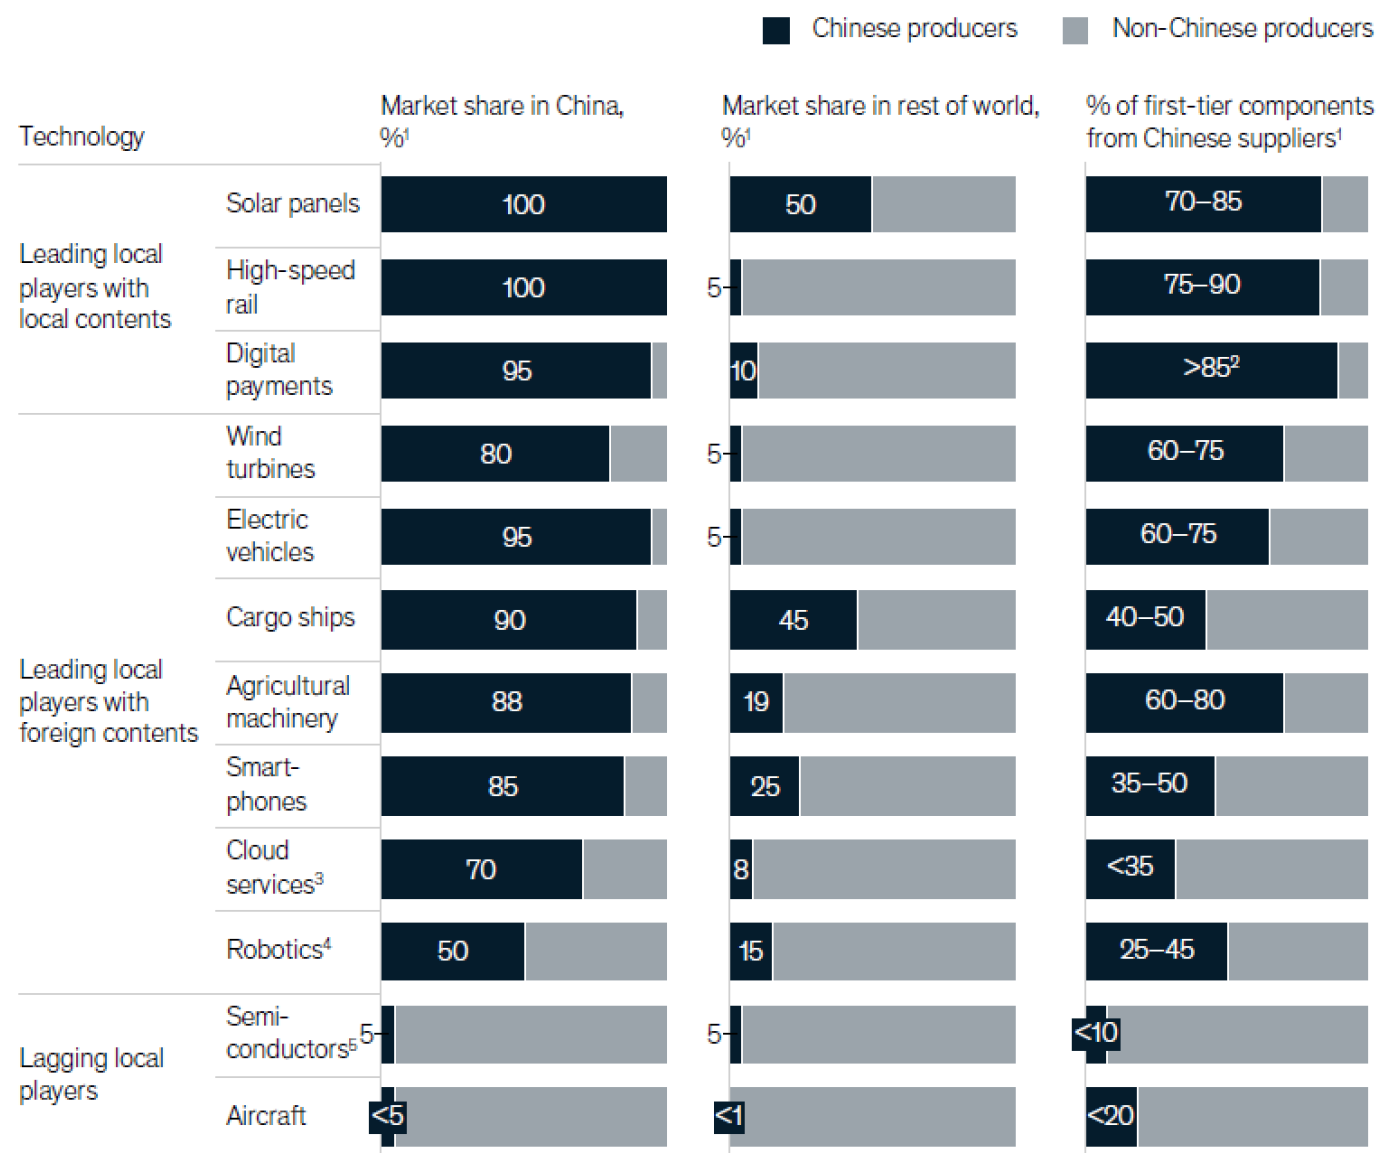
\includegraphics[width=0.7\textwidth]{Pictures/china_trade_2.png}
\end{figure}

\begin{figure}[H]
    \centering
    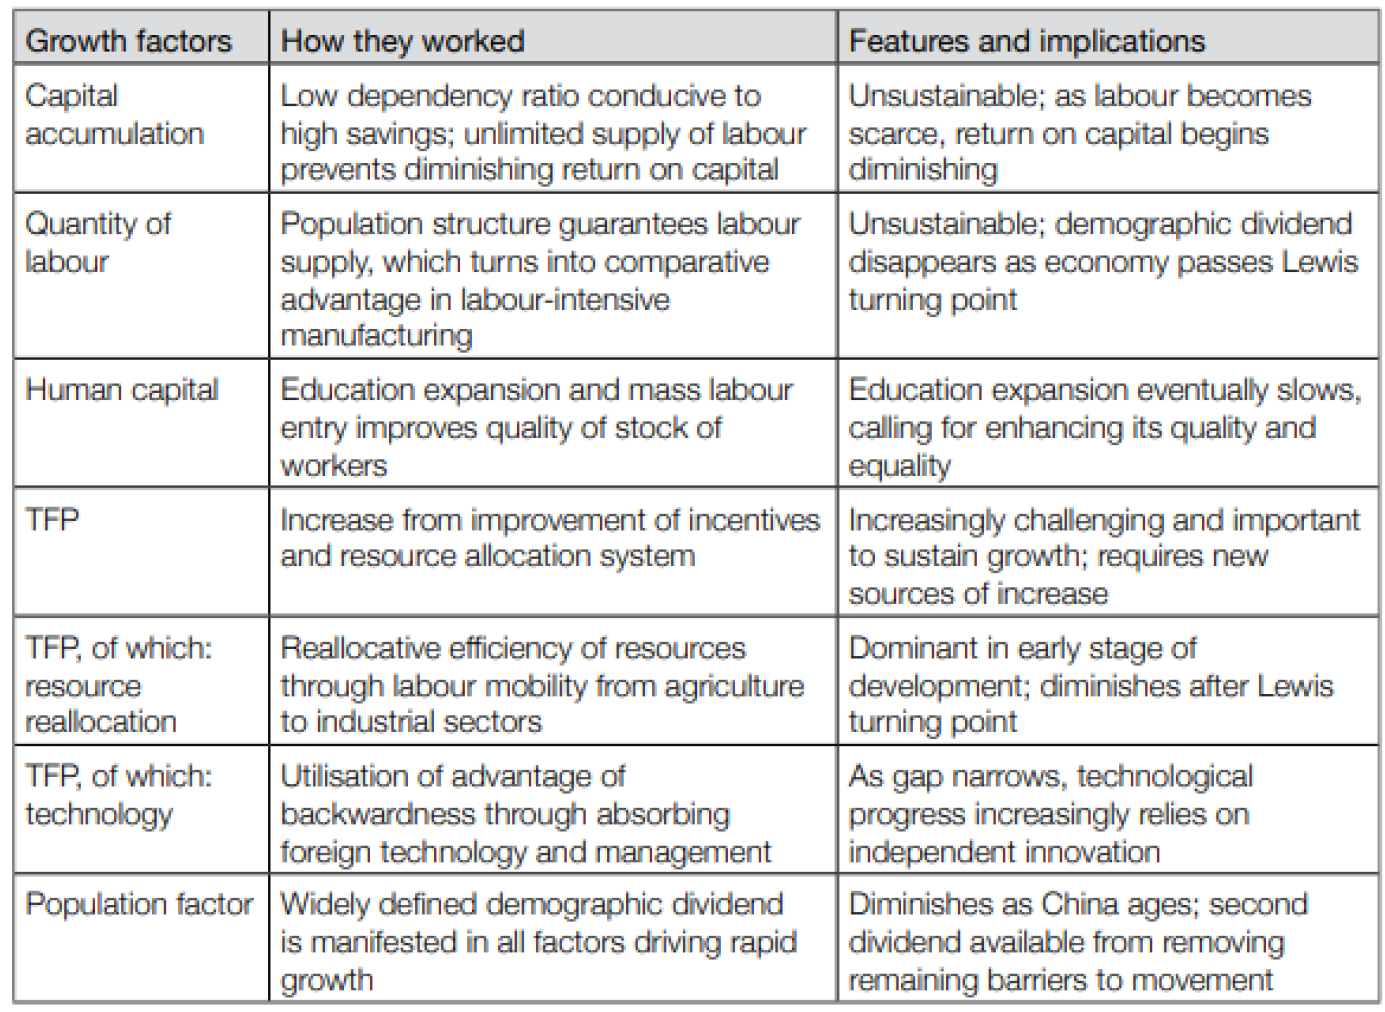
\includegraphics[width=0.8\textwidth]{Pictures/china_trade_summary.png}
    \caption{Summary Chinese Trade}
\end{figure}

\subsection{China is an old superpower with a recent brief dent (How China fell
and woke up)}

History of China: Ancient China and Century of Humiliation (1839-1949).
People's Republic of China: 1949-1978 and 1979-now.

\begin{figure}[H]
    \centering
    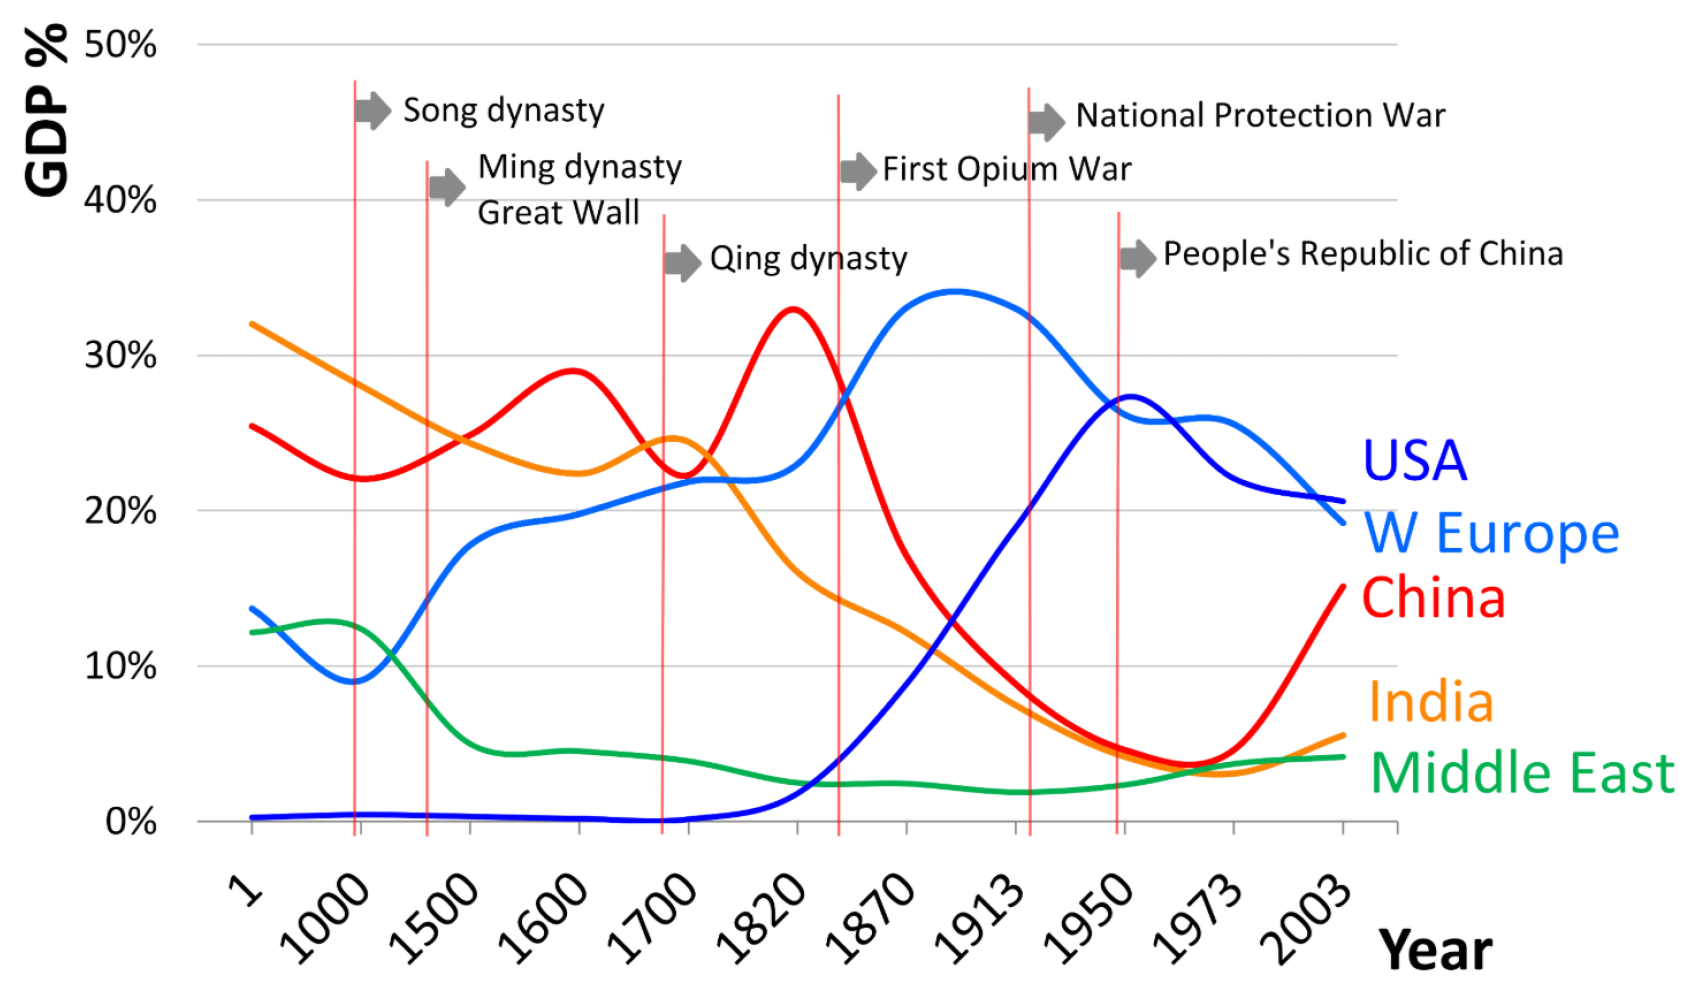
\includegraphics[width=0.8\textwidth]{Pictures/GDP_time_china.png}
\end{figure}

The european explorer Marco Polo (1254-1324 CE) traveled on the trading routes
centered on the Silk Road and described them in depth in his famous work but
he is not credited with naming them. Both terms for this network of roads were
coined by the German geographer and traveler, Ferdinand von Richthofen, in
1877 CE, who designated them 'Seidenstrasse' (silk road) or 'Seidenstrassen'
(sild routes). Polo, and later von Richthofen, make mention of the goods which
were transported back and forth on the Silk Road.

\paragraph{Four great inventions}

\subparagraph{Paper Making}
In the early Western Han Dynasty, China invented papermaking.
Papermaking is a great revolution in writing materials.

\subparagraph{Printing}
In the early Tang Dynasta, engraving printing was invented from the
seals and engraving stone.

\subparagraph{Movable type printing}
In the early 11th century, Bi Sheng, a civilian in the Northern Song Dynasty,
invented movable type printing, which was more than four centuries earlier
than the European invention. The spread of North Korea and Japan to Egypt and
Europe to the west. The invention of printing is a major contribution to the
spread and preservation of human culture.

\subparagraph{Gunpowder}
It was invented by ancient alchemists in China, and the books in the middle
of Tang recorded the method of making gunpowder. It was used in the military
in the late Tang Dynasty. It was invented in the Southern Song Dynasty, and
was introduced into Arabia and Europe in the 13th century. The invention and
spread of gunpowder changed the medieval mode of warfare and was a major
event in the military era.

\subparagraph{Compass}
During the Warring States period, people made the instrument "Sinan" indicating
the direction, and later using the principle of magnet guide to make a compass.
In the Song Dynasty, the magnetized steel needle support was fixed in an
azimuth-engraved disk for pointing. This is the compas, also known as the
compas needle. The compass of the Northern Song Dynasty was used for navigation.
Introduced to Arabia and Europe in the 13th century. The invention and spread
of the 13th century. The invention and spread of the compass privided important
conditions for european navigators to explore new routes.

\subsubsection{Century of Humiliation (1839-1949)}

In this period, China suffered major international fragmentation, lost almost
all of the wars it fought, and was often forced to give major concessions to
the great powers in the subsequent treaties. In many cases, China was forced
to pay large amounts of reparations, open up ports for trade, lease or cede
territories and make various other concessions of sovereignty to foreign
"spheres of influence", following military defeats.

\begin{itemize}
    \item Defeat in the First Opium War (1839-1842) by the UK.
        \begin{itemize}
            \item Treaty of Nanking (Aug 1942): cession of Hong Kong; four
                additional "treaty ports" opened for foreign trade; 21 million
                dollars reparations (annual income 57 mio)
        \end{itemize}
    \item The Taiping Rebellion (1850-1864): One of the bloodiest wars in
        human history, the bloodiest civil war, and the largest conflict of
        the 19th century. Estimates of the war dead range from 10-30 million.
    \item Defeat in the Second Opium War (1856-1860) and the sacking of the
        Old Summer Palace by British and French forces.
    \item The Sino-French War (1884-1885)
    \item Defeat in the First Sino-Japanese War (1894-1895) by Japan
        \begin{itemize}
            \item Treaty of Shimonoseki (Apr 1895): recognized the indeppendence
                of Korea and renounced any claims to that country; ceded the
                Liaodong Peninsula, and the islands of Formosa (Taiwan) and
                Penghu (also known as Pescadores) to Japan; paid Japan a war
                indemnity of 200 million Kuping taels silver (7500 tonns),
                payable over seven years; opening of various ports and rivers to
                japanese trade.
        \end{itemize}
    \item The Eight-Nation Alliance (Austria-Hungary, France, Germany, Italy,
        Japan, Russia, the US and the UK) suppressing the Boxer uprising (1899-1901)
        \begin{itemize}
            \item Boxer Protocol (Sep 1901): 450 million taels of fine silver
                were to be paid as indemnity over 39 years to the eight naitons
                involved; to prohibit the importation of arms and ammunation; the
                destruction of Taku Forts; Legatin Quarters occupied by the
                Power shall be considered as a special area reserved for their
                use under exclusive control, in which Chinese shall not have the
                right to reside, and which may be defensible; concede the right
                to the Powers to station troops in 12 cities/places; Boxer and
                Governments or their nationals.
        \end{itemize}
    \item British expedition to Tibet (1903-1904)
    \item The Twenty-One Demands (1915) by Japan
    \item Japanese invasion of Manchuria (1931-1932)
    \item The Second Sino-Japanese War (1937-1945): 15-22 million death
\end{itemize}


The Moa Era (1949-1977): Mao Zedong's tenure as Chairman of the PRC triggered
sweeping changes for the country.

\begin{itemize}
    \item 1953-1957: First 5-Year Plan: The program's aim was to boost
        China's industrialization. Steel production grew four-fold in four
        years, from 1.3 million tonnes to 5.2 million tonnes. Agriculture
        output also rose, but it couldn't keep pace with industrial production.
    \item 1958-1962: Great Leap Forward: The campaign emphasized China's
        agrarian-to-industrial transformation, via a communal farming system.
        However, the plan failed - causing an economic breakdown and the deaths
        of tens of millions in the great Chinese Famine.
    \item 1959-1962: Lushan Conference and 7000 Cadres meeting:
        Top leaders in the Chinese Communists Party (CCP) met to create
        detailed policy frameworks for the PRC's future.
    \item 1966-1976: Great Proletarian Cultureal Revolution:
        Mao Zedong attempted to regain power and support after the failures
        of the Great Leap forward. However, this was anoter plan that backfired,
        causing more deaths by violence and again crippling the Chinese economy.
    \item 1971: Joined the UN: The PRC replaced the ROC (Taiwan) as a permanent
        member of the UN. This addition also made it one of only five members
        of the UN Security Council - including the UK, the U.S., France, and
        Russia.
    \item 1972: President Nixon's visit: After 25 years of radio silence,
        Richard Nixon was the first sitting US President to step foot into the
        PRC. This helped re-establish diplomatic relations between the two nations.
    \item 1976-1977: Mao Zedong Death, and "Two Whatevers": After Mao Zedong's
        passing, the interim government promised to "resolutely uphold whatever
        policy decisions Chairman Mao made, and unswervingly follow whatever
        instructions Chairman Mao gave."
    \item 1979: "One-Child Policy": The government enacted an aggressive
        birth-planning program to control the size of country's population,
        which it viewed as growing too fast.
    \item When the PRC (People's Republic of China) was established in
        1949, China accounted for 4.2\% of the global economy, but this
        number increased to only 4.9\% by 1978. In 1949, GDP per capita was
        \$23, and was \$156.4 in 1968.
\end{itemize}

Before 1978 the leaders were more ideologistic. After, no matter which
regime, as long as it works.

\paragraph{Reform and development strategy}
Justin Yifu Lin and Zhongkai Shen (2018). In China's 40 Years of Reform and
Development 1978-2018.
\begin{itemize}
    \item Why was China able to achieve such extraordinary growth during
        its transition? Why was China able to grow so dynamically during the
        reform period? Answer: The latecomer advantage.
    \item Why was China unable to attain similar success before its
        transition started? If the latecomer advantage was the reason
        for China's extraordinary growth performance after 1978, the same
        advantage should have existed for centuries before 1978, so why did
        China not benefit before the reform and opening-up? Answer: Because
        China voluntarily gave up the latecomer advantage.
    \item Why did few other transitional economies perform equally well?
        Answer: Because other economies followed the wrong transition strategy:
        the neoliberal 'Washington consensus', which was based on the argument
        that the misallocation of resources caused by excessive government
        intervention led to unsatisfactory economic performance. 'shock therapy'.
        China adopted a pragmatic, gradual and dual-track approach.
\end{itemize}

\subsection{China is a Confucious dominant country (East and West culture difference)}

\begin{itemize}
    \item Shower: West: Morning, East: evening
    \item Waiting Queue: West: line, East: bunch of people
    \item Way of life: West: indipendence and individualism, East: community oriented
    \item Restaurant: West: calm, East: noisy
    \item Punctuality: West accurate, East: flexible
    \item Opinions: West: straight forward, East: complicated
    \item Making Contacts: West: linear relationships with few people, East: circular relationships across many people
    \item Anger/Displeasure: West: If unhappy, emotions can be perceived through body language etc,
        East: Norm is to hide displeasure
    \item View of Myself: West: most important, East: part of the sum.
    \item Handling Problems: West: most direct approach, East: involve indirect approach
    \item The Boss: West: weaker influence, East, great authority and influence as well as respect.
    \item Truth: West: honest, East: liar
    \item Talking about Money: West: no problem, East: not appropriate to talk about money
\end{itemize}

\subsubsection{Confucianism}
The main foundations of Confucianism emphasize duty, sincerity, loyalty,
honor, filial piety, respect for age and seniority. As individuals maintain
harmonious relations among themselves, society itself becomes stable.
\begin{itemize}
    \item Balance
    \item Hamony
    \item Modest
    \item Hierarchy
    \item Seniority
    \item Internal Hamony
\end{itemize}
Chinese business culture is largely influenced by Confucianism.
The Confucian concept of Guanxi means that a relationship network is crucial
and based on the values of solidarity, loyalty, modesty and courtesy.
Hierarchy in China, both in business and privacy, is purely vertical and highly
respected. Chinese people will be careful to save face in order to protect
individual reputations, influence and dignity. Some of these values have
slowed down over the last decade and modern Western business approaches are
gaining ground.

\paragraph{Collectivism vs. Individualism}
This is referred to as the degree to which individuals in a certain country
prefer acting as individuals rather than as members of groups. This dimension
focuses on the relationship between the individual and the larger social
groups.

It encourages people to pull up their socks and get out of poverty. On the
other hand, China as collectivistic society encourages more group work and
puts more emphasis on strong relationship between individuals hence the basis
of guanxi. To them, the needs of a group are way more important than
individual needs.

\paragraph{Characteristics of Individualistic Cultures}

\begin{itemize}
    \item Fosters contractual relationships that revolve around the basics
        of exchange. In such cultures, calculation of the profit or loss
        of engaging in a particular behaviour is calculated before going
        for it.
    \item Concentrates more on self and the very dear or near ones as well as
        concern with behavioural relationships as well as own interests, needs
        and own goals.
    \item More emphasis on personal pleasure, over duties, fun, enjoyment and
        social norms. They are part of in-groups, but they hardly have any
        influence on their lives.
    \item Value independence and self-sufficiency with self-interest placement
        rather than collective interests. In such societies, confrontation is
        an acceptable attribute.
    \item They hold unique beliefs and decisions are made based on individual
        needs.
\end{itemize}

\paragraph{Characteristics of Collectivistic Cultures}

\begin{itemize}
    \item For maintenance of social harmony among in-group members, the
        behaviour must subscribe to the social norms established.
    \item More giving up of personal interests and sharing of resources to
        facilitate the colllective interests.
    \item Before making any major decision must consider the implications to
        the wider collective.
    \item Favoritism expecially to in-groups including family and friends.
    \item Be a part of few influential in-groups and inclining towards
        conformality.
    \item Increased concern when it comes to ingroup members but show indifference
        or hostility towards out-group members.
    \item Much emphasis on hierarchy and harmony within the group.
    \item There are group norms which help in the regulation of behaviour.
\end{itemize}

\paragraph{FACE}
\begin{itemize}
    \item One of the central concepts in Chinese social life is 'face' (mianzi)
        because China is a collectivistic society in which social harmony is of
        utmost importance.
    \item Face reflects one's social self-esteem and the way one is regarded in
        society and interpersonal interactions.
    \item People can 'have face' as long as they are respected by others, but
        they can 'lose face' when they experience a public embarrassment.
    \item Public disagreement is a face-losing act of the Chinese: they prefer
        articulating the intentions in an indirect manner and leaving room for
        negotiations in private. Enhancing or saving others' face helps
        tremendously in building friendships and creating interpersonal goodwill.
    \item Face-saving actions sometimes are the cost of precision, accuracy, and
        clarity and may become compatible with honest or truthful communication
        practices.
\end{itemize}

\paragraph{Communication}

\begin{itemize}
    \item To Westerners, the word 'yes' suggests agreement and affirmation, but
        to Chinese a 'yes' may only convey the meaning of 'I am listening' with
        the purpose of showing attention and politeness.
    \item Chinese way of communication focuses on different elements, including
        implicit, context-based, listening-centered, and face-oriented mathods.
    \item Unlike the Western communication pattern, Chinese prefer to use an
        implicit language pattern - meaning is often implied of must be inferred.
    \item Also, they tend to take context and the specific situation into account
        when interpreting a word. So the ability to surmise and decipher hidden
        meanings is highly desirable in Chinese culture.
\end{itemize}

\paragraph{Modesty}

\begin{itemize}
    \item Chinese people value modesty and humbleness.
    \item To grow up as a Chinese, one learns not to take credit for one's
        behaviour or be boastful in any situation.
    \item Self-effacing/other-enhancing is common rule in Chinese socialization process.
    \item When receiving a compliment such as 'your son is an excellent boy',
        a Chinese would automatically say 'not really'.
    \item In Chinese culture, blatantly accepting a compliment is considered impolite.
    \item However, young Chinese professionals do not tend to keep a low profile.
        They tend to be more confident, self-expressive and direct.
\end{itemize}


\subsection{China in internally highly heterogenous and complex}

China often seems like a nonolith of 1.3 billion people, but it's not. It's
a mosaic of distinct regions, and understanding those regions is vital to
understanding China.

The Chinese are people with diverse physical traits, dialects and traditions.
They are multicultural, multireligious, and a multiethnic society, having
as many as 55 ethic groups as diverse and interesting as the geography and
the history of the country they inhabit. Several of them are descendant of
Arabs who came here via the Silk Road in early centuries.

\begin{itemize}
    \item Language: 8 main variants of spoken Chinese and hundreds of less common ones
    \item 56 Ethnicity
    \item Regional Stereotypes
    \item Economic development
\end{itemize}

\begin{figure}[H]
    \centering
    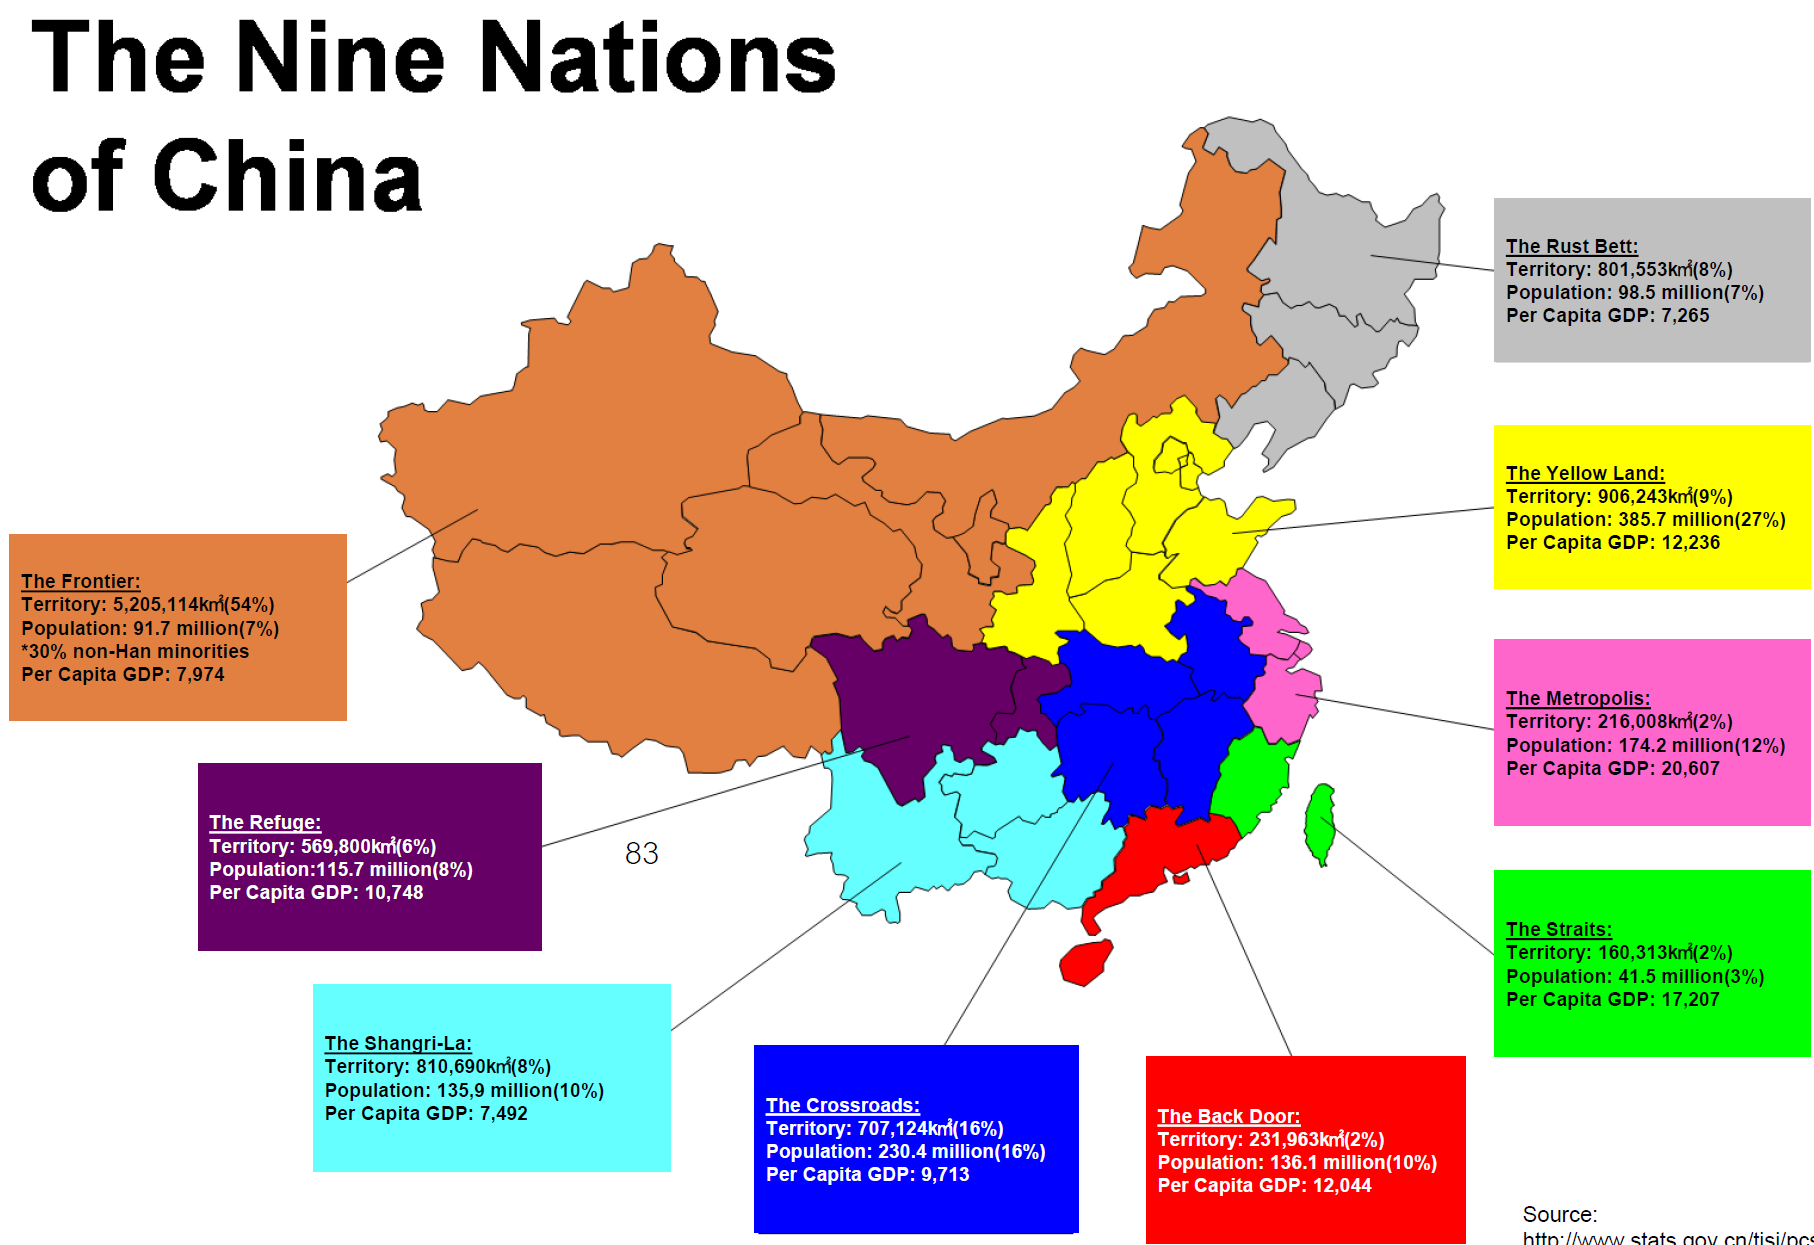
\includegraphics[width=0.9\textwidth]{Pictures/The_nine_nations_of_china.png}
    \caption{The nine nations of China}
\end{figure}

\begin{figure}[H]
    \centering
    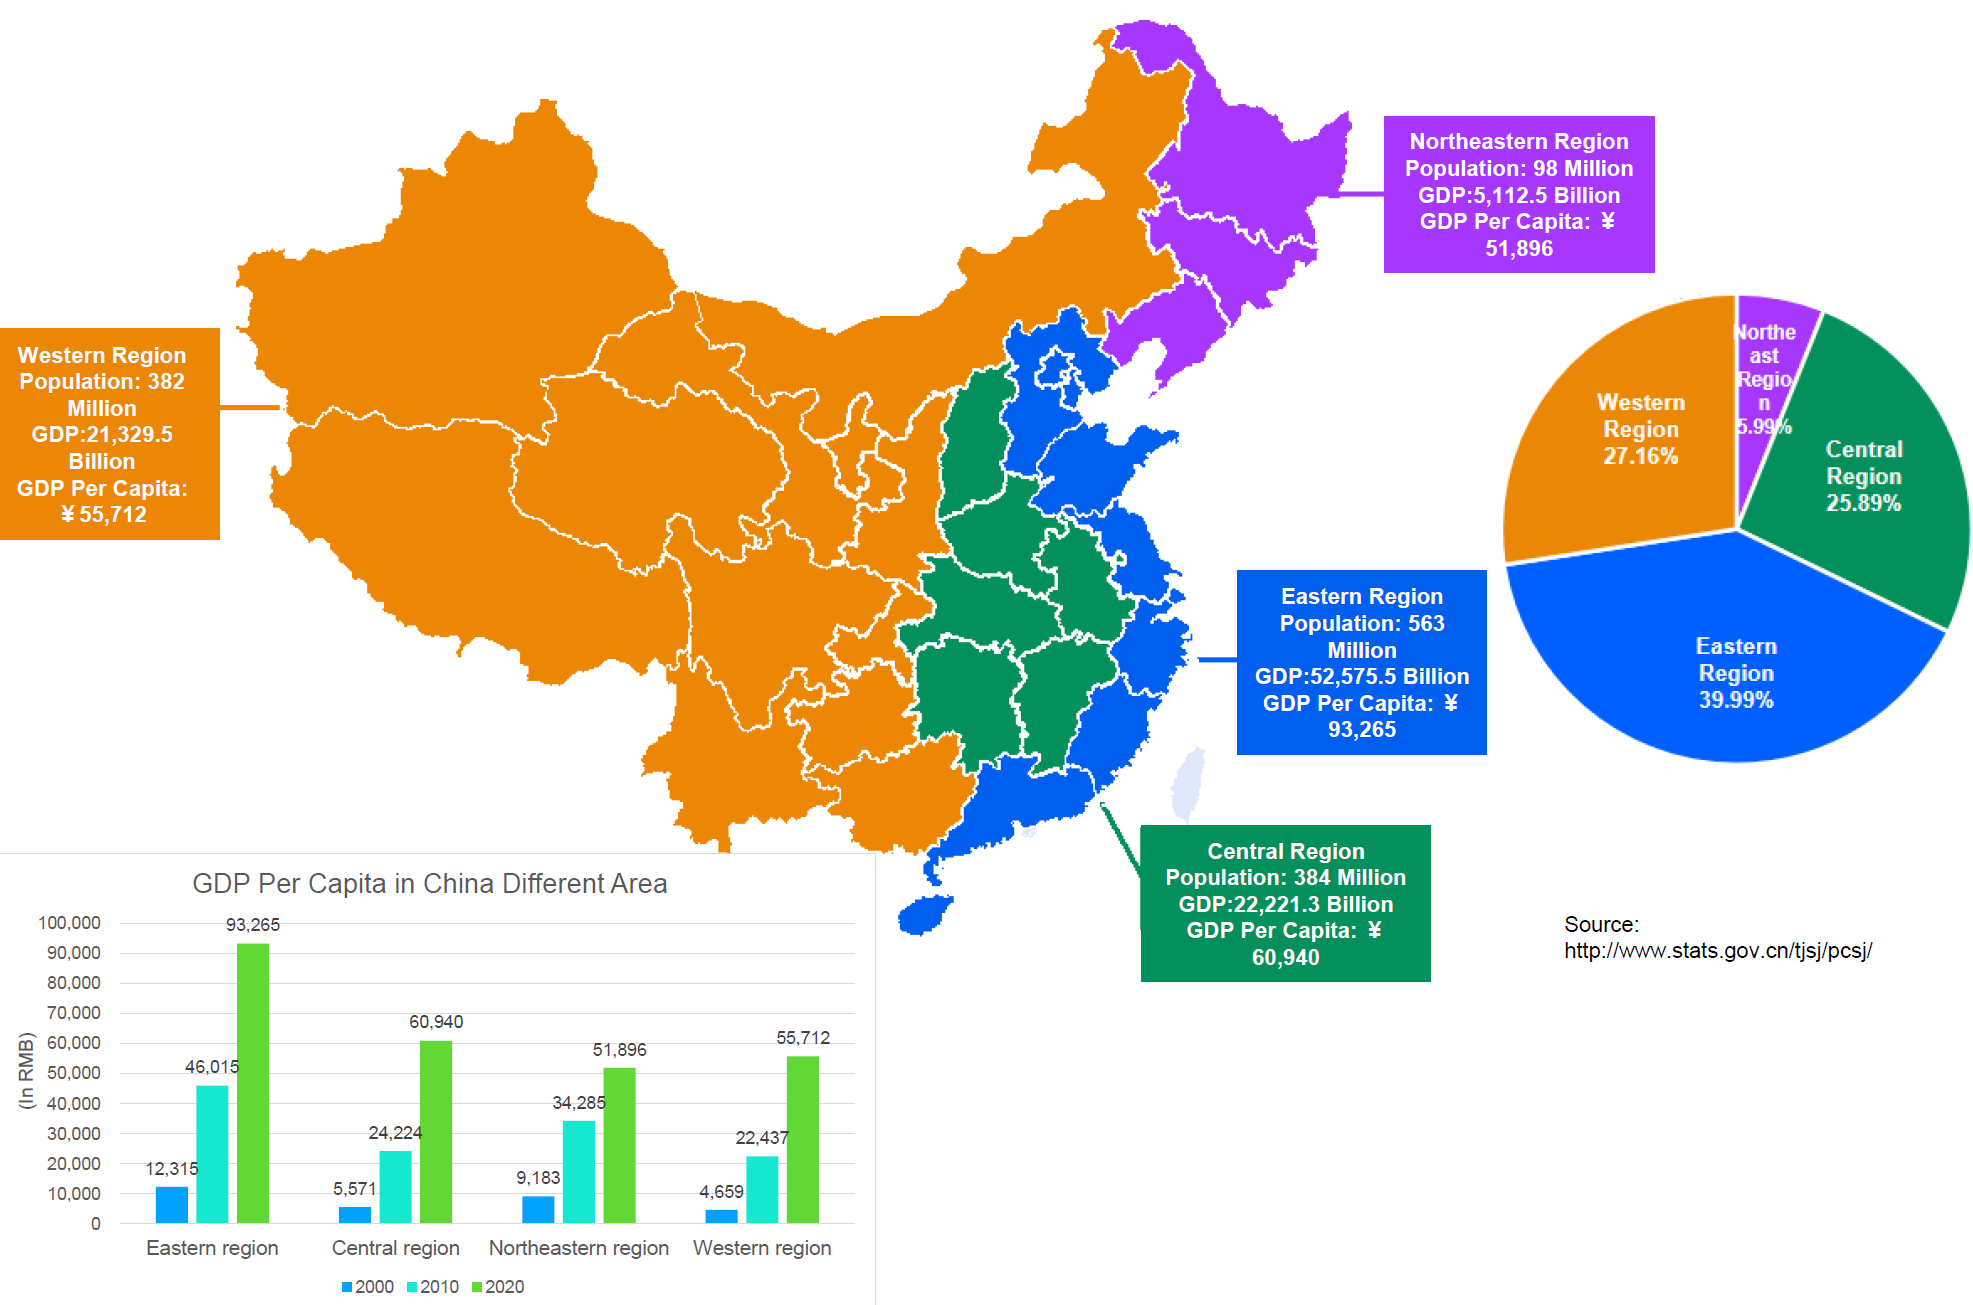
\includegraphics[width=\textwidth]{Pictures/The_nine_nations_of_china_2.png}
\end{figure}

There is a strong corrolation between political freedom and economic succes
of a country. Human societies must create stable sources of food energy, or
they die out. The ability to access saable sources of food energy is a function
of the available technology for growing, storing, and transporting food crops.
Given any particular state of technology, brute facts of nature determine the
amount of accessible food energy by affecting what can be grown, how much of it
can be grosn, whether it can be stored, and the distance at which it can be
traded.

\paragraph{4 Complex Adaptive Systems}

\begin{itemize}
    \item Transactional Complex Adaptive Systems
        \begin{itemize}
            \item Produce, relatively large fertile land, idiosyncratic weather shocks
            \item Shock $\Rightarrow$ move and trade $\Rightarrow$ rule of law and democratic system
        \end{itemize}
    \item Insurance Complex Adaptive Systems
        \begin{itemize}
            \item Produce, relatively large fertile land, aggregate weather shocks
                (massive shock lasting for years)
            \item Centralized coordination system
        \end{itemize}
    \item Subsistence Complex Adaptive Systems
        \begin{itemize}
            \item Produce but not be able to store (tropics with rainfall)
            \item No trade $\Rightarrow$ no surplus $\Rightarrow$ no investment
                in human capital and other infrastructural systems $\Rightarrow$ bands/tribes
        \end{itemize}
    \item Pastoral Complex Adaptive Systems
        \begin{itemize}
            \item Not possible to produce enough kilocalories $\Rightarrow$
                expand, move to outrun aggregate weather shocks (Steppe ecosystems)
        \end{itemize}
\end{itemize}
